\documentclass[a4paper]{report}

%====================== PACKAGES ======================

\usepackage{fullpage}

\usepackage[french]{babel}
\usepackage[utf8]{inputenc}
\usepackage[T1]{fontenc}

\usepackage{hyperref}
\hypersetup{
	colorlinks=true,
	linkcolor=black,
        urlcolor=black,
}

\usepackage{amsfonts, amsmath, amsthm, mathtools}
\usepackage{setspace}
\usepackage{graphicx}

\usepackage{listings, xcolor}
\definecolor{codegray}{rgb}{0.5,0.5,0.5}
\definecolor{codepurple}{rgb}{0.58,0,0.82}
\definecolor{backcolour}{rgb}{0.95,0.95,0.92}
\lstdefinestyle{mystyle}{
    backgroundcolor=\color{backcolour},
    commentstyle=\color{codegray},
    keywordstyle=\color{orange},
    numberstyle=\tiny\color{codegray},
    stringstyle=\color{codepurple},
    basicstyle=\ttfamily\footnotesize,
    breakatwhitespace=false,
    breaklines=true,
    frame=single,
    captionpos=b,
    keepspaces=true,
    numbers=left,
    numberstyle=\footnotesize,
    stepnumber=1,
    numbersep=10pt, 
    showspaces=false,
    showstringspaces=false,
    showtabs=false,
    tabsize=4,
    linewidth=0.83\linewidth,
    xleftmargin=2cm,
}
\lstset{style=mystyle}

\usepackage{theoremref}
\theoremstyle{plain}
\newtheorem*{theorem}{Théorème}
\newtheorem*{definition*}{Définition}
\newtheorem*{proposition}{Proposition}
\theoremstyle{definition}
\newtheorem{example}{Exemple}

%======================== INTRODUCTION ========================

\makeindex
\onehalfspacing
\bibliographystyle{prsty}

%======================== DEBUT DU DOCUMENT ===================

\begin{document}

%======================== FIRST PAGE ==========================

    \begin{center}
    
        
\includegraphics[width=0.5\textwidth]{media/logo_upc.pdf}
        \vfill
        {\Large \textsc{Projet mathématiques - Informatique}\par}
        \vspace{1.5cm}
        {\huge\bfseries Factorisation des grands nombres\par}
        \vspace{2cm}
        {\Large Aggoun Tara, Aziz Ghizlane\par}
        Encadré par \textsc{Brunat Olivier}
        \vfill
        {\large Mai \the\year \par}
        \vspace{2cm}

    \end{center}
    
    \tableofcontents
    \newpage

%======================== CHAPTERS ==========================

    \chapter*{Introduction}
    \addcontentsline{toc}{chapter}{Introduction}
    Le chiffrement RSA tient son nom de ses trois inventeurs, Ronald Rivest, Adi Shamir et Leonard Adleman.
Il s'agit d'un algorithme de cryptographie asymétrique inventé en 1977. Cet algorithme est utilisé pour sécuriser la transmission de données sur Internet. \\

L'algorithme repose sur le principe mathématique de la factorisation des nombres premiers, plus précisément, sur le fait qu’il est très simple de multiplier deux nombres entiers, alors qu’il est extrêmement difficile de retrouver les deux facteurs si on ne connaît que le produit. Il utilise une paire de clés, représentée par des nombres entiers, composée d'une clé publique pour chiffrer les données et d'une clé privée pour les déchiffrer. La clé publique est accessible à tout le monde, tandis que la clé privée est gardée secrète par le destinataire des données.\\

Le chiffrement RSA est considéré comme sûr car il est très difficile de factoriser de grands nombres premiers en utilisant les algorithmes existants. Il est pratiquement impossible pour une personne ne possédant pas la clé privée de décrypter les données ainsi chiffrées. C'est pourquoi cette technique est utilisée pour protéger par exemple des transactions financières ou bien des communications sensibles sur les réseaux informatiques. \\

Dans ce projet, on étudiera différentes méthodes pour factoriser des nombres. On abordera également un test de primalité, qui permet de détecter si un nombre est premier sans avoir à montrer explicitement qu’il ne possède aucun diviseur non trivial.\\

Nous avons décidé d'implémenter nos algorithmes en Python, car il ne fixe pas de bornes pour la tailles des entiers, à la différence d'un grand nombre de langages de programmation.

\section*{Notation}
    Dans la suite du rapport on va utilisé les notations suivante:
    \begin{itemize}
        \item $\lfloor . \rfloor$ est la  partie entiere inférieur.
        \item $\mathbb{Z}/2\mathbb{Z}$ est le corps à deux élements, que l'on note $\overline{0}$ et $\overline{1}$.
        \item $\overline{m}$ désigne la classe de m dans $\mathbb{Z}/2\mathbb{Z}$.
    \end{itemize}

    \chapter{Méthode des divisions successives}
    \input{chapters/divisions_successives}

    % \chapter{Méthode p - 1 de Pollard}
    % \input{chapters/p-1_pollard}

    % \chapter{Méthode rho de Pollard}
    % \input{chapters/rho_pollard}

    \chapter{Méthode de Fermat}
    La méthode de Fermat a été trouvée par le mathématicien français Pierre de Fermat.
Elle est très efficace pour factoriser n, si n s’écrit comme un produit de deux entiers proches l’un de l’autre.
Elle repose sur le fait que déterminer une factorisation de n est équivalent à écrire n comme une différence de deux carrés. \\

Le principe de cette méthode est de trouver un u tel que $(\lfloor \sqrt{n} \rfloor + u) ^ 2 - n$ 
est un carré que l’on va noter $s^2$. 
On note aussi $r = \lfloor \sqrt{n} \rfloor + u$.
Une fois trouvés notre r et notre s, on va pouvoir factoriser n car on a :
       \[r^2 - n = s^2 ~~ \Leftrightarrow ~~ n = (r - s) (r + s)\] \\
Afin de déterminer u, on examine successivement les entiers 
\[\lfloor \sqrt{n} \rfloor + 1, ~ \lfloor \sqrt{n} \rfloor + 2, ~ ...\]

Voici notre implémentation de la méthode de Fermat:
\begin{lstlisting}[language=Python]
def _find_a_b(n): 
    (b, root) = _is_square(n)
    if b == 1: 
        return (root, root)
    for u in range (1, ((n + 1) // 2) + 1):
        r = root + u
        (b, s) = _is_square((r * r) - n)
        if b == 1: 
            return (r - s, r + s)
    return (n, 1)

def all_divider(n, facteurs={}):
    (a, b) = _find_a_b(n)
    if a == n or b == n:
        facteurs[n] = facteurs.get(n, 0) + 1
    else:
        utils.merge_dicts(facteurs, all_divider(a, facteurs))
        utils.merge_dicts(facteurs, all_divider(b, facteurs))
    return facteurs
\end{lstlisting}
\vspace{1em}

\newpage
Nous avons ici deux fonctions, la première, \lstinline{_find_a_b} qui prend en paramètre le nombre qu'on veut factoriser, \lstinline{n}. 
Cette fonction va retourner deux facteurs de n en utilisant la méthode de Fermat.
La deuxième fonction \lstinline{_all_divider} qui prend en arguments \lstinline{n}, le nombre à factoriser, et \lstinline{facteurs}, le dictionnaire qui va contenir tous les facteurs de n. Elle va appeler \lstinline{_find_a_b} qui permet de trouver deux facteurs et va s'appeler récursivement pour chercher tous les facteurs.
De plus, une fonction auxiliaire est appelée, \lstinline{_is_square(n)}, qui renvoie un couple, la première valeur vaut 1 si n est un carré parfait et la seconde est sa racine carrée; sinon elle renvoie -1 et la valeur absolue de sa racine carrée.

\begin{example}
   Grâce à cette méthode, nous parvenons à factoriser n = 399772198733 en moins de deux secondes.
   En effet nous commençons par vérifier que n n'est pas un carré parfait. \\ 
   On a que \[\lfloor \sqrt{n} \rfloor = 632275\]
    Ensuite on itère sur u jusqu'à ce que $(\lfloor \sqrt{n} \rfloor + u) ^ 2 - n$, soit un carré, ce qui arrive pour  \[u = 4022\]
    On a donc \[r = 636297 ~ \textrm{et} ~ s = 71426 \textrm{,}\]
    et on obtient \[399772198733 = 564871 \times 707723\]

    Maintenant, nous allons recommencer cette procédure sur les deux facteurs:\\
    Pour n = 564871, on trouve :
    \[u = 281685\]
    \[r = 282436 ~ et ~ s = 282435\]
    Donc \[564871 = 1 \times  564871\]
    Ainsi 564871 est premier. \\

    De la même façon, pour n = 707723, on trouve :
    \[u = 353021\]
    \[r = 353862 ~ et ~ s = 353861 \textrm{.}\]
    Donc \[707723 = 1 \times  707723\textrm{,}\]
    ce qui prouve que 707723 est premier. \\

    On a bien à la fin que \[399772198733 = 564871 \times 707723\]
    
\end{example}

    \chapter{Le crible quadratique}
    La principe du crible quadratique a été inventée par C. Pomerance en 1981. 
C’est aujourd’hui la méthode la plus couramment utilisée pour factoriser des entiers n qui n’ont pas de diviseurs premiers significativement plus petits que $\sqrt{n}$. 
Elle ne dépend en fait que de la taille de n, et non de propriétés arithmétiques particulières de ses diviseurs premiers.\\

Afin de factoriser n, on recherche des congruences modulo n entre carrés, c'est-à-dire que l'on cherche des entiers dont la différence de leurs carrés soit un multiple de n, et ne vaut pas n.
Supposons que l'on ait deux entiers u et v tels que: \[u^2 \equiv v^2 [n] ~ avec ~ u \not\equiv \pm v [n]\textrm{.}\]
Dans ce cas, on peut obtenir très simplement une factorisation de n, vu que n divise $(u - v)(u + v)$ sans diviser $u - v$ ni $u + v$. Le calcul des entiers \[pgcd(u - v, n) ~ et ~ pgcd(u + v, n)\] fournit alors des diviseurs non triviaux de n.\\

\begin{definition*}\label{polynome de Kraitchik}

On introduit alors le polynôme de Kraitchik, \[Q(X) = X^2 - n \in \mathbb{Z}[X]\]
    
\end{definition*}

\begin{definition*}[friabilité]\label{friable}
    Soit B un entier naturel. On dit qu'un entier est B-friable si tous ses diviseurs premiers sont inférieurs ou égaux à B.\\
    
\end{definition*}
Le but va être de trouver une suite d'entiers $x_1, ~ ..., ~ x_k$ avec  $k > \pi(B)$ tel que $Q(x_1), ~ ..., ~ Q(x_k)$ sont B-friables et 
\[Q(x_1) ~ ... ~ Q(x_k) = v^2 ~ ou ~ v\in \mathbb{N}\] et \[u = x_1 ~ ... ~ x_k.\]
On a alors \[u^2 \equiv (x_i^2 - n) ~ ... ~ (x_k^2 - n) = Q(x_1) ~ ... ~ Q(x_k) = v^2 ~ [n].\]
De plus, il y a une grande probabilité que $u \not\equiv \pm v$ \\

La difficulté est donc de trouver ces $x_k$. 
Pour cela, nous allons commencer par déterminer quelle valeur prendre pour notre B de la B-friabilité. Si B est trop petit, cela risque d'être compliqué de conclure car on n'est pas sûr de parvenir à expliciter un seul entier x qui soit B-friable. Si B est trop grand, il faudra un très grand nombre de x, et on n'est pas sûr d'en trouver assez. Il faut trouver un juste milieu.
Le comportement asymptotique de B en fonction de n incite à choisir: \[B = exp(\frac{1}{2}\sqrt{log(n)log(log(n))})\]

Une fois que l'on a déterminé B, on cherche k entiers B-friables grâce à la \hyperref[B-friabilite]{méthode de recherche des entiers B-friables}.\\

Une fois que l'on a trouvé notre suite $x_k$ d'entiers, il va falloir choisir lesquels d'entre eux nous seront utiles pour la factorisation de n. Pour cela, nous allons appliquer le principe de la \hyperref[Matrices]{recherche de congruences de carrés}.\\

\begin{proof}
    Notons $p_1, ~ ..., ~ p_{\pi(B)}$ les nombres premiers inférieurs ou égaux à B.\\
    $\forall ~ 1 \leq j \leq k$, on a,
    \[Q(x_j) = \prod\limits_{i=1}^{\pi(B)} {p_i}^{n_{ij}} \textrm{, avec } n_{ij} \in \mathbb{N}\]
    on pose
    \begin{align*}
        \prod\limits_{j=1}^{k} Q(x_j) = \prod\limits_{j=1}^k {\prod\limits_{i=1}^{\pi(B)} {p_i}^{n_{ij}}}\\
        = \prod\limits_{i=1}^{\pi(B)} {{\prod\limits_{j=1}^k {p_i}^{n_{ij}}}}\\
        = \prod\limits_{i=1}^{\pi(B)} {{p_i}^{\sum\limits_{j=1}^k {n_{ij}}}}
    \end{align*}
 
    En particulier, $\prod\limits_{j=1}^{k} Q(x_j)$ est un carré ssi $\sum\limits_{i=1}^k {n_{ij}} \equiv 0 [2], ~ \forall ~ 1 \leq j \leq \pi(B)$\\
    
    ssi $\forall ~ 1 \leq j \leq \pi(B), ~ \sum\limits_{i=1}^k {\overline{n_{ij}}} = \overline{0}$, où $\overline{0}$ désigne la classe de 0 dans $\mathbb{Z}/2\mathbb{Z}$.
    
    Introduisons la matrice $M = (\overline{n_{ij}}) \in M_{\pi(B),k} ~ (\mathbb{Z}/2\mathbb{Z})$, la matrice contenant les puissances modulo 2 des $Q(x_i)$.\\
    Soit $X = 
    \begin{pmatrix}
        \alpha_1 \\ ... \\ \alpha_k
    \end{pmatrix}
    \in (\mathbb{Z}/2\mathbb{Z})^k$ tel que $X \in ker(M)$\\
    On a alors $\sum\limits_{j=1}^k {\alpha_j ~ \overline{n_{ij}}} = \overline{0}, ~ \forall ~ 1 \leq i \leq \pi(B)$.\\
    Notons $J = \left\{ j \in \left\{1, ..., k\right\} | \alpha_j = \overline{1} \right\}.$
    Alors \begin{align*}
        \sum\limits_{j=1}^k {\alpha_j \overline{n_{ij}}} = \overline{0} &\Longleftrightarrow \sum\limits_{j\in J} {\overline{n_{ij}}} = \overline{0} ~ \forall ~ 1 \leq i \leq \pi(B)\\
        &\Longleftrightarrow \sum\limits_{j\in J} {n_{ij}} ~ est ~ pair ~ \forall ~ 1 \leq i \leq \pi(B)\\
        &\Longleftrightarrow ~ \forall ~ 1 \leq i \leq \pi(B), ~ \exists ~ q_i \in \mathbb{N} ~ tq ~ \sum\limits_{j \in J} {n_{ij}} = 2 q_i
    \end{align*}
    Posons $u_J = \prod\limits_{j \in J} {x_j}$ et $v_J = \prod\limits_{i=1}^{\pi(B)} {{p_i}^{q_i}}$.\\
    On a alors 
    \begin{align*}
        {u_J}^2 = \prod\limits_{j\in J} {{x_j}^2} &\equiv \prod\limits_{j\in J} {Q(x_j) [n]}\\
        &\equiv \prod\limits_{i=1}^{\pi(B)} {{p_i}^{\sum\limits_{j \in J} {n_{ij}}} [n]}\\
        &\equiv \prod\limits_{i=1}^{\pi(B)} {{p_i}^{2q_i} [n]}\\
        &\equiv (\prod\limits_{i=1}^{\pi(B)} {{p_i}^{q_i})^2 [n]}\\
        &\equiv {v_J}^2 [n]
    \end{align*}
    Ainsi, à tout élément $X \in ker(M)$, on est en mesure d'associer deux éléments $u_J$ et $v_J$ tq ${u_J}^2 \equiv {v_J}^2 [n],$\\
    et qui ont une chance d'être tels que $u_J \not\equiv v_J [n]$
\end{proof}

Une fois que l'on a déterminé lesquels de nos $x_k$ nous seront utiles, on a enfin trouvé une factorisation de n, car nous avons \[v = \sqrt{Q(x_1) ~ ... ~ Q(x_k)}\] ainsi que: \[u = x_1 ~ ... ~ x_k\]
par ailleurs, au moins un de: \[pgcd(u - v, n) ~ et ~ pgcd(u + v, n)\] est un facteur de n. \\

Voici notre implémentation:\\

Nous avons une fonction \lstinline{_divider} qui prend en paramètre \lstinline{n}, le nombre à factoriser, et qui va chercher deux diviseurs non triviaux de n. 
Cette fonction utilise \lstinline{find_b} qui renvoie le B adéquat en fonction de n, \lstinline{eratosthene}, qui utilise \hyperref[Eratosthène]{le crible d'Eratosthène} pour trouver les nombres premiers inférieurs à B, et \lstinline{_find_2_divider} qui est expliqué dans \hyperref[Matrices]{l'annexe C}.
\clearpage
\begin{lstlisting}[language=Python]
def _divider(n):
    b = utils.find_b(n)
    primes = ce.eratosthene(b)
    k = len(primes) + 1
    (fct1, fct2) = (1, 1)
    while(1):
        (fct1, fct2) = _find_2_divider(n, primes, k)
	if fct1 != 1 or fct2 != 1:
		break
	k += 1
    return (fct1, fct2)
\end{lstlisting}
\vspace{1em}

\begin{example}
    Essayons de factoriser 2041.\\
    On commence par chercher B. On trouve B = 7.\\
    et tous les nombres premiers inférieurs ou égaux à B sont
    \[[2, 3, 5, 7]\]
    On cherche donc k > $\pi(7) = 4$. \\
    On trouve donc grâçe à la \hyperref[B-friabilite]{recherche des entiers B-Friables} 6 entiers, dont leurs images par le \hyperref[polynome de Kraitchik]{polynôme de Kraitchik} sont 7-friables.
    \[[46, 47, 49, 51, 53, 54]\]
    avec leurs images
    \[75 = 3 \times 5^2, ~ 168 = 2^3 \times 3 \times 7, ~ 360 = 2^3 \times 3^2 \times 5, ~ 560 = 2^4 \times 5 \times 7, ~ 768 = 2^8 \times 3, ~ 875 = 5^3 \times 7\]

    À partir de ces 6 entiers et de la \hyperref[Matrices]{recherche de congruences de carrés.}
    On trouve cette matrice

    \[\begin{pmatrix}
    0 & 1 & 1 & 0 & 0 & 0\\
    1 & 1 & 0 & 0 & 1 & 0\\
    0 & 0 & 1 & 1 & 0 & 1\\
    0 & 1 & 0 & 1 & 0 & 1
    \end{pmatrix}\]

    dont le noyau est engendré par
    \[\begin{pmatrix} 1\\ 0\\ 0\\ 0\\ 1\\ 0\end{pmatrix} \textrm{ , } \begin{pmatrix} 1\\ 1\\ 1\\ 0\\ 0\\ 1\end{pmatrix}\textrm{.}\]

    Nous allons utiliser le premier vecteur, On doit ainsi utiliser notre premier entier qui est 46 et le 5eme qui est 53.
    On a \[u = 46 \times 53 = 2438\]
    et \[v^2 = 75 \times 768 = 2^8 \times 3^2 \times 5^2\]
    Donc \[v = 2^4 \times 3 \times 5 = 240\]
    on a ainsi \[u + v = 2678 ~ et ~ u - v = 2198\]
    on calcule \[pgcd(2678, 2041) = 13 ~ et ~ pgcd(2198, 2041) = 157\]
    on en conclut que \[2041 = 13 \times 157\]
    Avec le \hyperref[Miller_Rabin]{test de primalité Miller Rabin} on trouve que 13 et 157 sont premiers, on a donc fini.
\end{example}


    % \chapter{Un algorithme optimisé}
    % \input{chapters/optimisé}

    % \chapter*{Conclusion}
    % \addcontentsline{toc}{chapter}{Conclusion}
    % \input{chapters/conclusion}

%======================== APPENDIX ========================
    \appendix

    \chapter{Le crible d'Ératosthène}
    \label{Eratosthène}
    Le crible d'Ératosthène qui, comme son nom l'indique, a été créé par Ératosthène, est un algorithme qui permet de trouver tous les nombres premiers inférieurs à un entier naturel N. \\
        
Le principe de ce crible est de prendre un tableau contenant tous les entiers de 2 a N.
On commence par rayer tous les multiples de 2 du tableau. 
On continue en procédant de la même façon avec le premier entier non rayé, ici 3. On continue jusqu'à atteindre $\sqrt{N}$. Tous les éléments non rayés du tableau sont premiers.\\

Voici notre implémentation du crible d'Eratosthène:
\begin{lstlisting}[language=Python]
def _smaller_n(n): 
	res = []
	i = 0
	while i <= n:
		res.append(i)
		i += 1
	return res
    
def _find_prime(n): 
    primes = _smaller_n(n)
    primes[0] = -1
    primes[1] = -1
    for i in range(2, utils.isqrt(len(primes)) + 1): 
        for j in range(i + 1, len(primes)): 
            if primes[i] != -1 and primes[j] % primes[i] == 0: 
                primes[j] = -1
    return primes

def eratosthene(n):
    tmp = _find_prime(n)
    res = []
    for i in range (len(tmp)): 
        if tmp[i] != -1: 
            res.append(tmp[i])
    return res
\end{lstlisting}
\vspace{1em}

Nous avons trois fonctions, la première, \lstinline{_smaller_n} qui prend en paramètre un entier \lstinline{n}, et va créer un tableau avec tous les entiers compris entre 0 et n. \\
La deuxième fonction, \lstinline{_find_prime}, qui prend en paramètre un entier \lstinline{n}, va récupérer le tableau de la précédente fonction et va le parcourir en mettant des $-1$ aux cases avec un indice non premier. \\
La dernière fonction \lstinline{eratosthene} prend en paramètre n et va renvoyer un tableau avec toutes les valeurs différentes de $-1$ contenues dans le tableau de \lstinline{_find_prime}. \\

\begin{example}
    Essayons de trouver tous les nombre premiers compris entre 0 et 30.
    Tout d'abord nous devons créer un tableau contenant tous les entiers entre ces bornes:
    \[[0, 1, 2, 3, 4, 5, 6, 7, 8, 9, 10, 11, 12, 13, 14, 15, 16, 17, 18, 19, 20, 21, 22, 23, 24, 25, 26, 27, 28, 29, 30]\]

    Nous mettons -1 aux indices 0 et 1 car il ne sont pas premiers. Et nous commençons par enlever tous les multiples de 2
    \[[-1, -1, 2, 3, -1, 5, -1, 7, -1, 9, -1, 11, -1, 13, -1, 15, -1, 17, -1, 19, -1, 21, -1, 23, -1, 25, -1, 27, -1, 29, -1]\]
    Une fois cela effectué, nous prenons le premier entier différent de -1 et supérieur à notre ancien pivot, ici 3. Nous enlevons ensuite tous ses multiples du tableau
    \[[-1, -1, 2, 3, -1, 5, -1, 7, -1, -1, -1, 11, -1, 13, -1, -1, -1, 17, -1, 19, -1, -1, -1, 23, -1, 25, -1, -1, -1, 29, -1]\]

    Nous procédons ainsi jusqu'à $\lfloor \sqrt{n} \rfloor = 5$ et nous obtenons:
    \[[-1, -1, 2, 3, -1, 5, -1, 7, -1, -1, -1, 11, -1, 13, -1, -1, -1, 17, -1, 19, -1, -1, -1, 23, -1, -1, -1, -1, -1, 29, -1]\]

    Une fois fini nous enlevons tous les $-1$ du tableau et nous avons tous les nombres premiers plus petits que 30:
    \[[2, 3, 5, 7, 11, 13, 17, 19, 23, 29]\]
\end{example}

    \chapter{Recherche des entiers B-Friable}
    \label{B-friabilite}
    Pour la recherche des entiers \hyperref[friable]{B-friables} de l'intervalle [1, X], on construit au départ un tableau contenant tous les entiers entre 1 et X. 
Pour chaque nombre premier $p \leq B$, on parcourt le tableau, en commençant avec l’entier p et, en effectuant successivement des pas de longueur p, on divise par p tous les entiers possibles dans le tableau, qui ne sont autres que les multiples de p plus petits que X. 
On obtient alors un nouveau tableau d’entiers entre 1 et X qui diffère du précédent seulement aux cases d’entiers multiples de p. 
En commençant avec l’entier p, qui est maintenant à la case $p^2$, et en effectuant successivement des pas de longueur $p^2$, on divise de nouveau par p tous les entiers possibles du nouveau tableau. 
On procède de même jusqu’à la plus grande puissance de p inférieure à X. 
Lorsque l’on a effectué ce processus pour tous les nombres premiers $p \leq B$, on obtient un tableau dans lequel les cases où se trouvent le chiffre 1 sont exactement celles du départ des entiers B-friables.\\

Dans notre implémentation de la recherche des entiers B-friable, on a dû procéder d'une façon analogue. Nous recherchons, pour un entier, s'il est B-friable.
Pour cela, on prend un entier naturel n et, pour chaque nombre premier $p \leq B$, on divise n par p jusqu'à ce que n ne soit plus un multiple de p. Une fois cela accompli, pour chaque p, si n vaut 1, il est B-Friable, sinon il ne l'est pas.

Voici notre implémentation:
\begin{lstlisting}[language=Python]
def is_friable(n, primes): 
    facteurs = {}
    cur = n
    for prime in primes:
        while cur % prime == 0:
	   cur = cur // prime
	   if prime in facteurs:
	       facteurs[prime] += 1
	   else :
	       facteurs[prime] = 1
	   if cur == 1:
	       return (True, facteurs)
    return (False, {})
\end{lstlisting}
\vspace{1em}

Nous avons donc \lstinline{is_friable} qui prend un entier n et un tableau de nombres premiers \lstinline{primes}, et qui, pour chaque nombre premier dans primes, va enlever toutes les puissances de ce nombre à n.
Cette fonction renverra \lstinline{True} et sa décomposition en facteurs premiers s'il est friable et \lstinline{False} avec le dictionnaire vide sinon.

\begin{example}
Essayons de trouver tous les entiers 10-friables entre 2 et 30: 
\[[2, 3, 4, 5, 6, 7, 8, 9, 10, 11, 12, 13, 14, 15, 16, 17, 18, 19, 20, 21, 22, 23, 24, 25, 26, 27, 28, 29, 30]\]
On va diviser une première fois par 2,
\[[1, 3, 2, 5, 3, 7, 4, 9, 5, 11, 6, 13, 7, 15, 8, 17, 9, 19, 10, 21, 11, 23, 12, 25, 13, 27, 14, 29, 15]\]
Puis encore jusqu'à ce qu'il n'y est plus de puissances de 2 dans le tableau
\[[1, 3, 1, 5, 3, 7, 1, 9, 5, 11, 3, 13, 7, 15, 1, 17, 9, 19, 5, 21, 11, 23, 3, 25, 13, 27, 7, 29, 15]\]
On continue avec le premier entier différent de 1, ici 3:
\[[1, 1, 1, 5, 1, 7, 1, 1, 5, 11, 1, 13, 7, 5, 1, 17, 1, 19, 5, 7, 11, 23, 1, 25, 13, 27, 7, 29, 5]\]
puis avec 5
\[[1, 1, 1, 1, 1, 7, 1, 1, 1, 11, 1, 13, 7, 1, 1, 17, 1, 19, 1, 7, 11, 23, 1, 1, 13, 27, 7, 29, 1]\]

Et enfin avec 7
\[[1, 1, 1, 1, 1, 1, 1, 1, 1, 11, 1, 13, 1, 1, 1, 17, 1, 19, 1, 1, 11, 23, 1, 1, 13, 1, 1, 29, 1]\]

On en conclut que,
\[[11, 13, 17, 19, 22, 23, 26, 29]\]
sont les seuls entiers non 10-friable entre 2 et 30.
\end{example}

    \chapter{Recherche de congruences de carrés}
    \label{Matrices}
    On se donne une suite de $x_k$ pour lesquels on cherche une sous-famille non vide telle que le produit des image des $x_i$ par le \hyperref[polynome de Kraitchik]{polynôme de Kraitchik} est un carré.\\

Le principe est de récupérer la décomposition en facteurs premiers des différents $x_k$ lors de notre \hyperref[B-friabilite]{recherche des entiers B-friables}. 
À partir de cela, on crée une matrice, où chaque colonne représente un  des $x_k$, chaque ligne est un des nombres premiers plus petits que B et, dans chaque case, va être inscrite la puissance du facteur modulo 2.\\

Une fois notre matrice créée, nous allons calculer son \hyperref[Noyau]{noyau}. 
Avec celui-ci, nous prenons un des vecteurs. Si à la position i il y a un 1 c'est que nous devons prendre le $x_i$ tandis que s'il y a un 0 c'est que nous n'en avons pas besoin.\\

Grâce à cela nous avons déterminé les entiers dont nous aurons besoin pour notre factorisation.\\

\begin{proposition}
    Nous sommes sûr de trouver une solution, si on a $k > \pi(B)$.
\end{proposition}

\begin{proof}
    Soit M, la matrice créée.\\
    Par le théorème du rang, on a \[dim(ker(M)) + dim(Im(M)) = k.\]
    D'où $\hspace{4.5cm}dim(ker(M)) = k - dim(Im(M))\vspace{2mm}$\\
    Or $\hspace{6cm}Im(M) \subseteq {(\mathbb{Z}/2\mathbb{Z})}^{\pi(B)}\vspace{2mm}$\\
    donc $\hspace{5cm}dim(Im(M)) \le \pi(B)\vspace{2mm}$\\
    Ainsi $\hspace{6cm}-\pi(B) \le - dim(Im(M))\vspace{2mm}$\\
    et $\hspace{6cm}k - \pi(B) \le k - dim(Im(M))\vspace{2mm}$\\
    Finalement $\hspace{4cm}dim(ker(M)) \geq k - \pi(B) > 0\vspace{2mm}$\\
    Il y a donc bien des solutions non triviales.
\end{proof}

Voici notre implémentation de la recherche de congruences carrées:
\begin{lstlisting}[language=Python]
def _find_2_divider(n, primes, k):
	(x_k, q_x_k) = _find_friables(n, primes, k)
	mat = _create_mat(q_x_k, primes)
	sols = resolution.resolution(mat)
	(fct1, fct2) = (1, 1)
	for sol in sols:
		u = []
		v2 = []
		for i in range(len(sol)):
			if sol[i] == 1:
				u.append(x_k[i])
				v2.append(q_x_k[x_k[i]])
		v = _sqrt_v(v2)
		(fct1, fct2) = kraitchik.Kraitchik(n, u, v)
		if (fct1 != 1 and fct1 != n) or (fct2 != 1 and fct2 != n):
			break
	fct1 = 1 if fct1 == 1 or fct1 == n else fct1
	fct2 = 1 if fct2 == 1 or fct2 == n else fct2
	return (fct1, fct2)
\end{lstlisting}
\vspace{1em}
La fonction \lstinline{_find_friables} renvoie un tableau contenant les entiers tels que leurs carrés sont B-friables et la décomposition en facteurs premiers de leurs carrés. \\
À partir de cette décomposition, nous pouvons créer la matrice, puis la résoudre.
Ensuite, on parcourt les différents vecteurs des solutions trouvées pour pouvoir en extraire des facteurs.

\begin{example}
    Prenons, n = 2041.\\ 
    Nous avons B = 7 donc primes = $[2, 3, 5, 7]$ et k = 5.\\
    On trouve six entiers 7-friables: $[46, 47, 49, 51, 53, 54]$
    avec la décomposition de leurs carrés: \[{46:\{3: 1, 5: 2\}, 47:\{2: 3, 3: 1, 7: 1\}, 49:\{2: 3, 3: 2, 5: 1\},51: \{2: 4, 5: 1, 7: 1\},53: \{2: 8, 3: 1\},54: \{5: 3, 7: 1\}}\]
    Avec ça nous en déduisons la matrice suivante, en mettant modulo 2 les puissances:
    \[\begin{pmatrix}
        0 & 1 & 1 & 0 & 0 & 0\\
        1 & 1 & 0 & 0 & 1 & 0\\
        0 & 0 & 1 & 1 & 0 & 1\\
        0 & 1 & 0 & 1 & 0 & 1
    \end{pmatrix}\]
    En calculant le noyau on trouve:
    \[\begin{pmatrix}
        1 & 1\\
        0 & 1\\
        0 & 1\\
        0 & 0\\
        1 & 0\\
        0 & 1
    \end{pmatrix}\]

    Nous avons donc deux possibilités pour trouver une factorisation.
    On peut soit utilser notre premier et notre cinquième entiers, soit utilisé notre premier, deuxième, troisième et sixième entiers
\end{example}

    \chapter{Résolution d'un système d'équations}
    \label{Noyau}
    Pour déterminer les solutions d'un système d'équations, nous allons calculer le noyau d'une matrice M.\\
Nous commençons par faire un pivot de Gauss pour réduire et échelonner notre matrice.
Le principe est de choisir un élément pivot dans la matrice, généralement le premier élément non nul de chaque ligne, et de l'utiliser pour éliminer les autres éléments de la colonne en soustrayant ou en ajoutant des multiples de la ligne du pivot aux autres lignes de la matrice. 
Le processus se poursuit jusqu'à ce que la matrice soit dans une forme échelonnée réduite, où les éléments au-dessus et en dessous de chaque pivot sont tous égaux à 0, et où chaque pivot est égal à 1.

voici notre implémentation du Pivot de Gauss:
\begin{lstlisting}[language=Python]
def pivot_de_gauss(mat):
    for i in range (len(mat)):
        if mat[i][i] != 1:
            for j in range (i + 1, len(mat)):
                if mat[j][i] == 1:
                    _switch_lines(mat, i, j)
                    break
        for j in range (len(mat)):
            if i == j:
                continue
            if mat[j][i] == 1:
                mat[j] = _xor_lines(mat[i], mat[j])
    return mat
\end{lstlisting}
\vspace{1em}
La fonction \lstinline{_switch_lines} échange les lignes i et j de la matrice.\\
La fonction \lstinline{_xor_lines} ajoute deux lignes dans $\mathbb{Z}/2\mathbb{Z}$.\\

Une fois notre matrice échelonnée réduite, il est simple de trouver les solutions.
Si une colonne i est remplie de zéros, on peut la supprimer de la matrice, et mettre dans la liste des vecteurs du noyau le vecteur qui vaut zéro partout et 1 à la position i.
Il suffit ensuite d'enlever l'identité, créée en échelonnant la matrice, et de la reporter aux colonnes restantes.

Voici notre implémentation,
\newpage
\begin{lstlisting}[language=Python]
def _add_col_vide(mat, col_vide):
	if col_vide == []:
		return _transpose(mat)

	for i in range(len(mat)):
		for num_col in col_vide:
			beg = mat[i][:num_col]
			end = mat[i][num_col:]
			mat[i] = beg + [0] + end

	res = []
	for num_col in col_vide:
		beg = mat[:num_col]
		end = mat[num_col:]
		res = beg + _get_line(num_col, len(mat[0])) + end

	return _transpose(res)
 
def resolution(mat):
	res = []
	mat = pdg.pivot_de_gauss(mat)
	(bol, num_col) = _is_col_zero(mat)
	col_vide = []
	while (bol == True):
		col_vide.append(num_col)
		mat = _remove_col(mat, num_col)
		(bol, num_col) = _is_col_zero(mat)
	mat = _remove_id(mat)
	mat = _add_id(mat)
	return _add_col_vide(mat, col_vide)
\end{lstlisting}
\vspace{1em}

\begin{example}
    Essayons de trouver le noyau de la matrice :
    \[\begin{pmatrix}
        0 & 0 & 1 & 1 & 0 & 1\\
        0 & 1 & 0 & 0 & 1 & 0\\
        0 & 0 & 1 & 0 & 1 & 1
    \end{pmatrix}\]
    Commençons par faire le pivot de Gauss:\\
    On voit que la première colonne est remplie de zéros. On cherche donc un pivot sur la deuxième colonne. \\
    On va alors échanger la première colonne et la deuxième : 
    \[\begin{pmatrix}
        0 & 1 & 0 & 0 & 1 & 0\\
        0 & 0 & 1 & 1 & 0 & 1\\
        0 & 0 & 1 & 0 & 1 & 1
    \end{pmatrix}\]
    Il y a déjà des zéros sur les autres lignes de la deuxième colonne.\\
    On passe ensuite à la troisième colonne qui a déjà un 1 à la deuxième ligne.
    Comme on ne veut pas de 1, à la troisième ligne, on va additionner les deux, modulo 2:
    \[\begin{pmatrix}
        0 & 1 & 0 & 0 & 1 & 0\\
        0 & 0 & 1 & 1 & 0 & 1\\
        0 & 0 & 0 & 1 & 1 & 0
    \end{pmatrix}\]
    Maintenant notre matrice est échelonnée, il ne nous reste plus qu'à la réduire en ajoutant à la deuxième ligne, la troisième, toujours modulo 2:
    \[\begin{pmatrix}
        0 & 1 & 0 & 0 & 1 & 0\\
        0 & 0 & 1 & 0 & 1 & 1\\
        0 & 0 & 0 & 1 & 1 & 0
    \end{pmatrix}\]

    Voilà notre pivot de Gauss effectué. \\
    On remarque que la premère colonne est remplie de zéros. 
    On peut donc la supprimer de la matrice et on ajoutera le vecteur avec le premier élément valant 1 à nos vecteurs appartenant au noyau.\\

    Nous avons maintenant la matrice:
    \[\begin{pmatrix}
        1 & 0 & 0 & 1 & 0\\
        0 & 1 & 0 & 1 & 1\\
        0 & 0 & 1 & 1 & 0
    \end{pmatrix}\]
    On supprime l'identité que nous avons sur les trois premières colonnes:
    \[\begin{pmatrix}
        1 & 0\\
        1 & 1\\
        1 & 0
    \end{pmatrix}\]
    et nous ajoutons l'identité sur les deux dernières lignes:
    \[\begin{pmatrix}
        1 & 0\\
        1 & 1\\
        1 & 0\\
        1 & 0\\
        0 & 1
    \end{pmatrix}\]
    Nous avons donc le noyau de la matrice:
    \[\begin{pmatrix}
        0 & 0 & 1\\
        1 & 0 & 0\\
        1 & 1 & 0\\
        1 & 0 & 0\\
        1 & 0 & 0\\
        0 & 1 & 0
    \end{pmatrix}\]
\end{example}

    \chapter{Test de primalité: Miller Rabin}
    \label{Miller_Rabin}
    Avant d'essayer de factoriser un entier n, on teste s'il n'est pas premier. 
Pour cela nous avons décidé d'utiliser le test de primalité probabiliste de Miller Rabin.

\begin{theorem}
    Soit n un nombre premier impair que l'on décompose sous la forme $n = 2^s \times d + 1$. 
    Alors n a la propriété suivante: pour tout entier a compris entre 1 et n - 1, alors
    \begin{itemize}
        \item ou bien $a^d \equiv 1 [n]$
        \item ou bien $\exists i$ dans $\left\{1, ..., s - 1\right\}$ tel que $a^{2^i d} \equiv -1 [n]$
    \end{itemize}
\end{theorem}

On peut déduire de ce théorème un test probabiliste.
Soit n, on écrit $n = 2^s \times d + 1$, et a compris entre 1 et n - 1.
On dit que n passe le test si,
    \begin{itemize}
        \item ou bien $a^d \equiv 1 [n]$
        \item ou bien $\exists i$ dans $\left\{1, ..., s - 1\right\}$ tel que $a^{2^i d} \equiv -1 [n]$
    \end{itemize}

Voici notre implémentation:
\begin{lstlisting}[language=Python]
def _millerrabin(n):
    if n <= 2: return True

    if n % 2 == 0: return False

    s = 0
    t = n - 1
    while 1:
        if t % 2 == 1: break
        t //= 2
        s += 1

    a = random.randint(2, n - 1)
    b = pow(a, t, n)
    if b == 1: return True

    for i in range(s):
        if b == n - 1: return True
        if b == 1: return False
        b *= b
        b %= n

    return False
\end{lstlisting}
\vspace{1em}
Un nombre premier passera le test quel que soit a, mais il y a des entiers composés qui le passeront pour un certain a. 
Donc si le test nous renvoie que l'entier n'est pas premier, nous sommes sûrs qu'il ne l'est pas. 
Tandis que s'il nous renvoie qu'il est premier, on a une probabilité de $\frac{1}{2}$ qu'il ne soit pas premier. \\

Pour réduire cette probabilité, on fait passer ce test plusieurs fois avec des entiers a différents. 
Nous avons décidé de faire passer le test 20 fois car on obtient une probabilité que le nombre ne soit pas premier, si les 20 tests nous indiquent qu'il l'est, de $\frac{1}{2^{20}} \simeq 9 \times 10^-7$. Cette probabilité est suffisamment petite pour nos tests.
\begin{lstlisting}[language=Python]
def is_prime(n):
    nb_test = 20
    for _ in range(nb_test):
        if not _millerrabin(n):
            return False
    return True
\end{lstlisting}
\vspace{1em}

\begin{example}
    Essayons de voir si 3132433 est premier, \\
    Tout d'abord décomposons n sous la forme $n = 2^s \times d + 1$, on obtient \[3132433 = 2^4 \times 195777 + 1\]
    Maintenant on tire un nombre aléatoire entre 2 et $n - 1$ $a = 1168143$
    on note \[b = a^d ~ [n] = 481284\]
    
    Comme b est différent de 1 ou de n - 1 modulo n, on calcule \[b^2 = 265605\] qui est toujours différent de n - 1.
    Donc on continue 
    \[b^4 = 492432 \textrm{, }  b^8 = 1371228\]
    Comme aucun de ces b ne vaut n - 1 modulo n, on en conclut que n n'est pas premier.
    
\end{example}

\begin{example}
    Testons pour n = 242377. \\
    Nous avons que  \[n = 2^3 \times 30297 + 1.\]
    Tirons aléatoirement $a = 22254$, on note\\
    \[b = a^d ~ [n] = 161923\]
    Comme b est différent de 1 ou de n - 1 modulo n, on calcule,
    \[b^2 = 168331 \textrm{, } b^4 = 242376.\]
    On a que $b^4$ = n - 1 modulo n.
    Par conséquent, n  a une probabilité de $\frac{1}{2}$ d'être premier.
\end{example}


    \chapter{Optimalité des algorithmes}
    \label{Graphique}
    Nous venons donc de voir trois algorithmes de factorisation.\\
Le premier est celui des divisions successives qui, comme nous l’avons expliqué précédemment, est efficace
pour trouver de petits facteurs.\\
Le deuxième est la méthode de Fermat, il est lui efficace quand les facteurs sont proches. \\
Le dernier, celui du crible quadratique, est le plus efficace quel que soit le nombre.\\
Nous avons donc essayé de les comparer pour voir lequel de ces algorithmes est le meilleur. \\
Pour se faire, on a généré 100 nombres aléatoires entre $1$ et $10^{20}$, puis tenté de les factoriser successivement par les
trois algorithmes. Le temps pris pour factoriser chacun des chiffres est modélisé par un graphe généré en Python. \\

Voici le résultat :\\
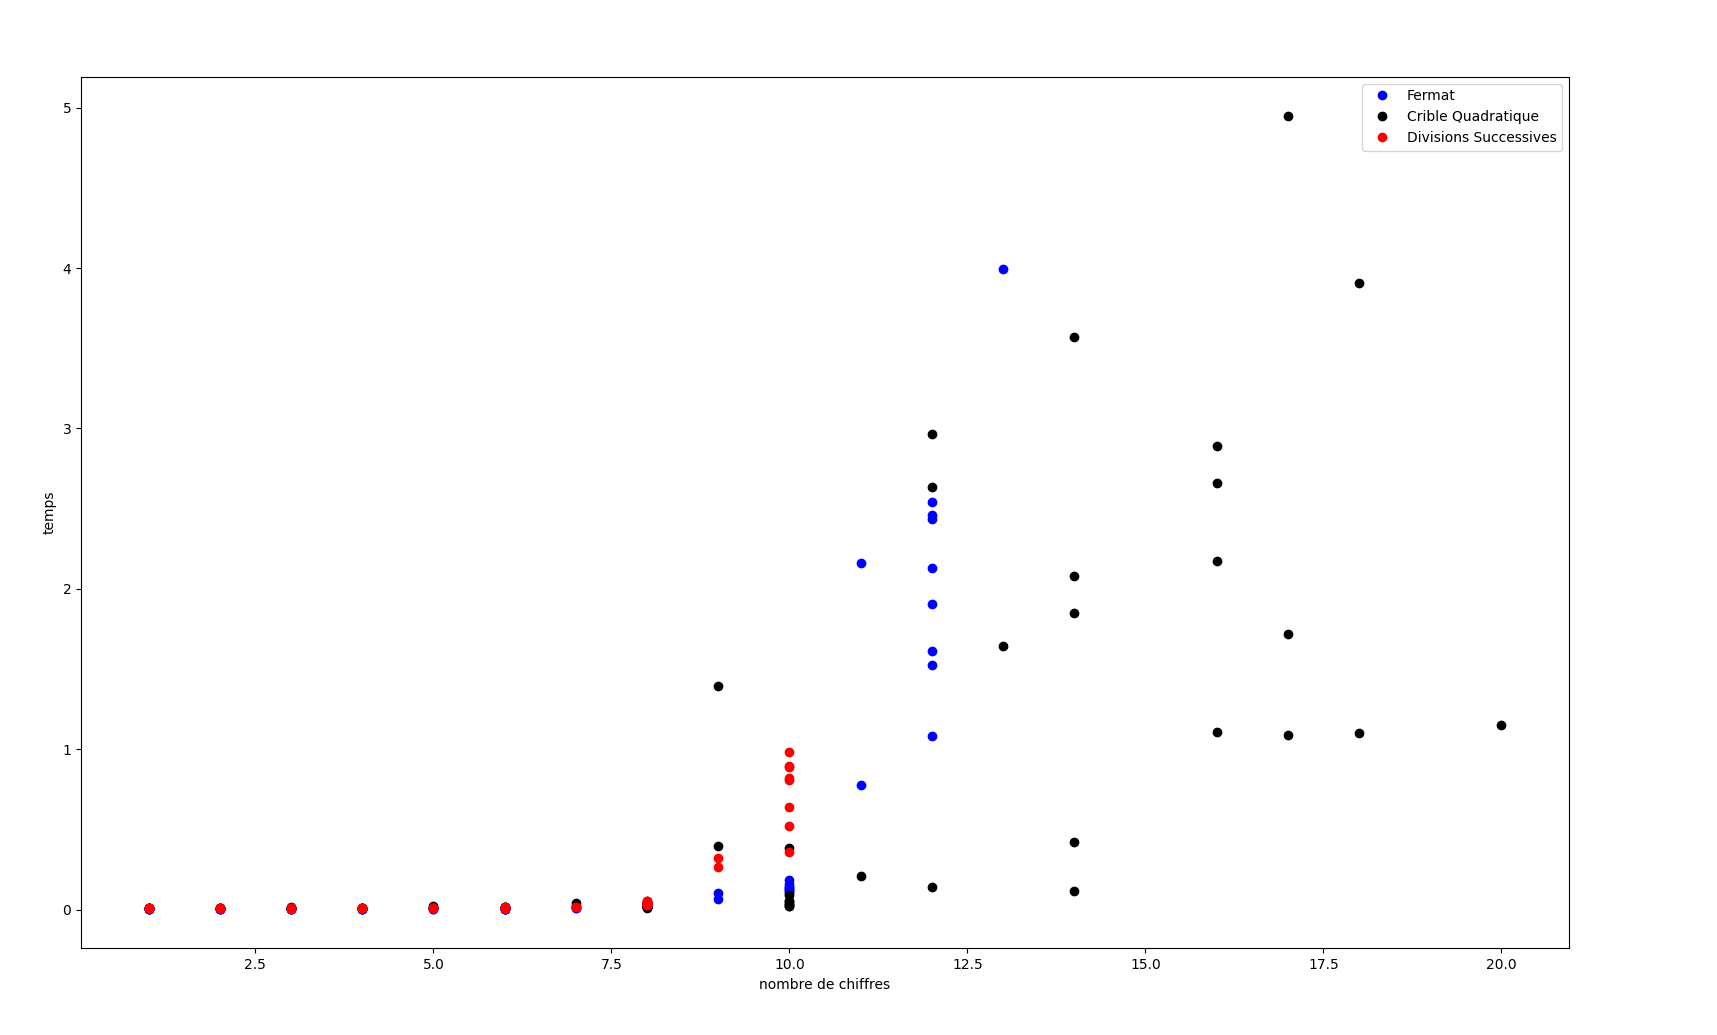
\includegraphics[width=0.75\textwidth]{media/4.png}\\
Si le temps de factorisation dépasse 5 secondes, on n’en tient pas compte et on passe au nombre suivant. \\
Ce graphe confirme nos prévisions : l’algorithme fondé sur le crible quadratique est le plus optimal. Il est en général plus rapide que les autres et il génère des solutions pour de plus grandes valeurs.
La méthode de Fermat est plus efficace que celle par divisions successives. Elle n'arrive cependant plus à factoriser à partir d’un nombre à 12 chiffres.La méthode par divisions successives quant a elle est la moins efficace. Elle échoue a factoriser un nombre s'il est supérieur à $10^{10}$.

    \chapter*{Bibliographie}
    \addcontentsline{toc}{chapter}{Bibliographie} 
        \begin{enumerate}

    	\item[[\,1\!\!]] \href{https://www.math.univ-paris13.fr/~boyer/enseignement/crypto/Chap6.pdf}{\textit{Méthodes de factorisation}, KRAUS Alain}
    	\item[[\,2\!\!]] \href{https://fr.wikipedia.org/wiki/Chiffrement_RSA}{Chiffrement RSA}
    	\item[[\,2\!\!]] \href{https://fr.wikipedia.org/wiki/Crible_d%27%C3%89ratosth%C3%A8ne}{Crible d'Eratosthene}
           
        \end{enumerate}

\end{document}
